\documentclass{webofc}
\usepackage[varg]{txfonts}   % Web of Conferences font
%
\begin{document}
%
\title{ATLAS Sim@P1 upgrades during long shutdown two}
%
\author{\firstname{Frank}
        \lastname{Berghaus}\inst{1}\fnsep\thanks{\email{berghaus@cern.ch}} \and
        \firstname{Franco} \lastname{Brasolin}\inst{2}\fnsep \and
        \firstname{Alessandro} \lastname{Di Girolamo}\inst{3}\fnsep \and
        \firstname{Marcus} \lastname{Ebert}\inst{1}\fnsep \and
        \firstname{Colin Roy} \lastname{Leavett-Brown}\inst{1}\fnsep \and
        \firstname{Chris} \lastname{Lee}\inst{4}\fnsep \and
        \firstname{Peter} \lastname{Love}\inst{5}\fnsep \and
        \firstname{Eukeni} \lastname{Pozo Astigarraga}\inst{3}\fnsep \and
        \firstname{Diana} \lastname{Scannicchio}\inst{6}\fnsep \and
        \firstname{Jaroslava} \lastname{Schovancova}\inst{3}\fnsep \and
        \firstname{Rolf} \lastname{Seuster}\inst{1}\fnsep \and
        \firstname{Randall}
        \lastname{Sobie}\inst{1}\fnsep\thanks{\email{sobie@uvic.ca}}
        \lastname{on behalf of the ATLAS Collaboration}
}
%
\institute{University of Victoria, Victoria, Canada
\and
           Universita e INFN, Bologna, Italy
\and
           CERN, Geneva, Switzerland
\and
           University of Cape Town, Cape Town, South Africa
\and
           Lancaster University, Lancaster, United Kingdom
\and
           University of California Irvine, Irvine, United States of America
          }
%
\abstract{%
  The Simulation at Point1 (Sim@P1) project was built in 2013 to take advantage
  of the ATLAS Trigger and Data Acquisition High Level Trigger (HLT) farm. The
  HLT farm provides around 100,000 cores, which are critical to ATLAS during
  data taking. When ATLAS is not recording data, this large compute resource is
  used to generate and process simulation data for the experiment. At the
  beginning of the current long shutdown (LS2), the HLT farm including the
  Sim@P1 infrastructure was upgraded. Previous papers emphasised the need for
  “simple, reliable, and efficient tools” and assessed various options to
  quickly switch between data acquisition operation and offline processing. In
  this contribution we describe the new mechanisms put in place for the
  opportunistic exploitation of the HLT farm for offline processing and give
  results from the first months of operation.
}
%
\maketitle
%
\section{Introduction}
\label{intro}
ATLAS~\cite{atlas} is a general purpose experiment located at point one (P1) of
CERN's large hadron collider. ATLAS employs a large computer farm, summarised in
table~\ref{tab:hlt_hardware}, to facilitate data acquisition and event
selection.
\begin{table}
\centering
\caption{The hardware at P1 currently available for use with Sim@P1. The C6100
nodes are the decommissioned old HLT. They provide 11008 hyper-threaded (HT)
cores permanently running in Sim@P1 mode. Not all cores are used to ensure the
virtual machines provide sufficient memory for ATLAS offline workloads. The
other hardware is switched to Sim@P1 mode when data taking is not foreseen in
the next 24 hours. These opportunistic resources provide up to 97216 additional
cores. Usually the trigger and data acquisition team retains some resources for
their needs.}
\label{tab:hlt_hardware}
\begin{tabular}{llllll}
\hline
Product name &
Intel\textsuperscript{\textregistered} Xeon\textsuperscript{\textregistered} &
HT cores & Memory [GB] & Instance cores & Nodes \\\hline
C6100 & X5650 & 24 & 24 & 16 & 688\\
Centerprise & E5-2650 v4 & 48 & 64 & 48 & 360 \\
Persy & E5-2660 v4 & 56 & 64 & 56 & 440 \\
MegWare & E5-2680 v3 & 48 & 64 & 48 & 680 \\
QuantaPlex & E5-2680 v3 & 48 & 64 & 48 & 472\\\hline
\end{tabular}
\end{table}
The Sim@P1 project aims to opportunistically use the trigger and data
acquisition high level trigger resources for offline computing. The High Level
Trigger (HLT)~\cite{tdaq2013} is a mission critical part of the ATLAS experiment
and is physically connected to the control network of the detector and the
``data'' network which allows connections to the CERN data centre through a
switch at P1. When working with Sim@P1 it is important to ensure the secure
isolation from the physical resources at P1, seamless integration into the ATLAS
distributed computing system, and reliable transition between the functions of
the resources. Throughout this text we will refer to standard operation of the
HLT as \textit{online mode} and the operation as part of the ATLAS distributed
computing system as \textit{offline mode}.

A system satisfying these criteria was developed during the first long shutdown
of the LHC~\cite{Ballestrero:2015ypa}. Isolation is achieved by running virtual
machines on the physical HLT hardware. The virtual machines were managed using
the cloud framework OpenStack~\cite{openstack}. The virtual machines share the
``data'' connection of the HLT hardware through a tagged VLAN providing network
isolation on the level of the Ethernet frame managed by the switches. This VLAN
allows the Virtual Machines to connect to a controlled list of interfaces in the
CERN general purpose network. This list specifies the interface of the machines
needed to allow offline workloads to be delivered and executed. To minimise
impact of Sim@P1 on the Trigger and Data Acquisition (TDAQ) operation, only
simulation tasks from the central production system are submitted to run at P1.

The original implementation of Sim@P1 ran successfully during the first long
shutdown of the LHC facilities between 2013 and 2015. Once the experiment
resumed data-taking, the system was used in opportunistic
mode~\cite{Ballestrero:2017psv}. The HLT was switched from TDAQ function to
Sim@P1 mode for intervals of a few days during technical stops and machine
development. To allow this opportunistic usage a set of scripts were developed
to manage the transition of resources between TDAQ and Sim@P1 mode.

During the second long shutdown (LS2) of the LHC facilities, starting in 2019,
the HLT
was be upgraded. The changes to the HLT necessitated an upgrade of the Sim@P1
infrastructure\footnote{The OpenStack Icehouse does not support operating on
CentOS7 running on the TDAQ HLT starting in 2019}. A previous
publication~\cite{Berghaus:2019wuj} offered multiple options for the upgrade of
the Sim@P1 infrastructure during the LS2. In this paper we describe how the
system was modified for operation with the upgraded HLT hardware.

\section{The Sim@P1 infrastructure}
\label{sec:infra}
During the year end technical stop from December 2017 to March 2018, the
computing hardware of the HLT was replaced with new nodes. The old HLT hardware
was retained at P1 and is permanently operating in offline. The new hardware has
been used offline during the various technical and machine development
stops throughout 2018. The current hardware configuration is summarised in
table~\ref{tab:hlt_hardware}.

When a HLT rack is not needed for data taking a shifter can set that rack to
offline operation. This action triggers a change in the configuration database
used by
the TDAQ. The next time the configuration management system runs on any server,
or trigger processing unit (TPU), in that rack\footnote{The configuration
management tool, Puppet, runs once an
hour on the TPUs.} it changes the system configuration to reflect the change
in the configuration database. When a TPU is in offline mode the configuration
management system ensures an ephemeral
disk providing 20~\textrm{GB} per core\footnote{Leaving at least 20\% of the
hard drive free.} exists and a virtual machine instance, based on a CernVM raw
image and this ephemeral disk, is running. This document will refer to such a
running virtual machine as an \textit{instance}.

Instances are contextualised using amiconfig\footnote{Originally a
project by rPath, Inc. now maintained by the CernVM team.}~\cite{amiconfig}.
The contextualisation is delivered using an ISO image added to the instance
by libvirt~\cite{libvirt}. The ISO image is formatted as an OpenNebula data
source. The
contextualisation sets up the computing environment for the ATLAS offline
workloads and sets the virtual machines to advertise themselves to a
HTCondor~\cite{condor} system running in the CERN general purpose network.
Instances are configured to use HTCondor's dynamic partitioning feature to
map workloads to the resources. Process isolation is achieved using cgroups.

The HTCondor system for Sim@P1 was rebuilt with a single central manager and
four schedulers. The virtual machines are managed by CERN's configuration
management system. Work is submitted to the schedulers using the PanDA
Harvester~\cite{harvester}. Sim@P1 presents a single unified production queue to
the PanDA system. The harvester is operating the queue in push mode allowing the
workloads to request the resources they need leveraging the dynamic partitioning
of workers.  The HTCondor system now directly notifies the PanDA workload
management system when resources are added or removed from Sim@P1.

\subsection{Content delivery}
CernVM is a good solution for Sim@P1 because the micro-image can be distributed
to all the TPUs and require a trivial disk space during HLT operation. Using
CernVM means that we rely on the CernVM file system (CVMFS) to provide both the
operating system content as well as the experiment software. In our CHEP2018
contribution we incorrectly stated that the load on the Frontier
squids during the switch to offline mode was low~\cite{Berghaus:2019wuj}.
This measurement was flawed in two ways: the instances were incorrectly
contextualised to retrieve the CVMFS content from the Frontier squids operated
by CERN IT for their batch system. Furthermore, the Frontier squids at P1 were
blocked by the Frontier servers, causing Frontier requests to fail over to the
CERN IT's squids Figure~\ref{fig:single_proxy} shows that, after correcting the
\begin{figure}[h]
\centering
\sidecaption
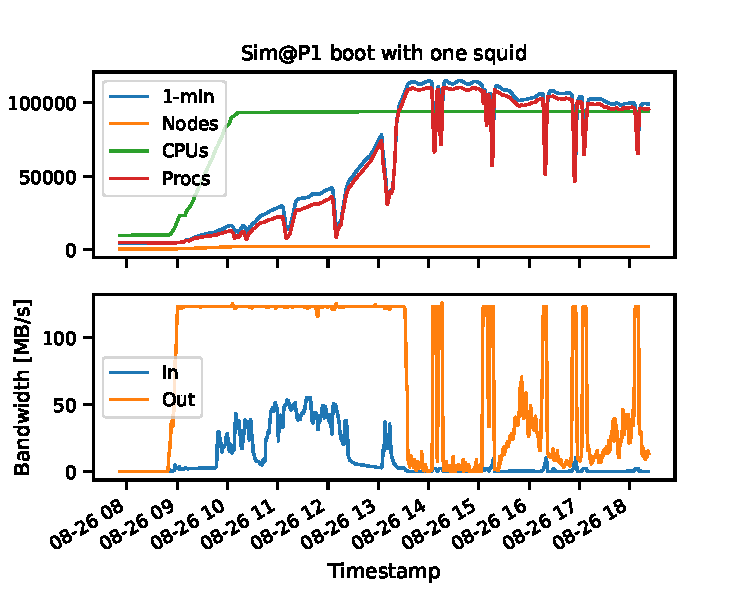
\includegraphics[width=0.6\textwidth,clip]{single_squid}
\caption{The top figure shows the number of instances, CPUs, and running
processes as well as the aggregate one minute load on the TDAQ HLT farm as it
transitions to Sim@P1 mode. Below, using the same timestamps, the network load
on the single Frontier proxy delivering the CVMFS content to all the nodes is
displayed. The correlation of saturated outgoing bandwidth in the lower plot
with
the steady increase in the load and processes in the upper plot suggests the
squid is the rate determining system in the transition of the farm.}
\label{fig:single_proxy}
\end{figure}
contextualisation, the Frontier squid at P1 was saturating its network bandwidth
to deliver the content required by the booting instances. To address the
bottleneck posed by the single squid we added a second squid instance,
then added CVMFS caches that persist throughout HLT operation, and finally
created
a hierarchy of squids on the instances in offline mode.

The addition of a second squid doubled to total bandwidth used to deliver the
content required for CVMFS. As a result the transition to Sim@P1 mode finished
in 3 hours - approximately twice as fast as with the single Frontier squid. In
the future we aim to replace the legacy hardware hosting the Frontier squids at
P1 with servers providing a factor of 10 more bandwidth.


\subsection{Persistent CVMFS caches}
\label{sec:cvmfs}
Much of the CVMFS content remains unchanged between successive switches between
offline and online mode. Updates to the operating system tend to be minimal. An
ATLAS software release are constant after being uploaded to CVMFS. So
persisting the CVMFS cache between periods of Sim@P1 operation should reduce the
amount of content the caches need to provide to booting instances.

A $50$~\textrm{GB} virtual disk image was created on each TPU to serve as
persistent CVMFS cache. The ephemeral disk may be smaller to
compensate for the size of the cache. Libvirt is configured to mount the cache
as an additional drive. The contextualisation checks for a second drive. If it
finds the second disk exists and is formatted with the label ``cache'' it
mounts the disk as the CVMFS cache. If the second disk exists but carries no
labelled partition the disk is formatted with the label ``cache'' and mounted.

Figure~\ref{fig:persistent_cache} shows that with a warm CVMFS cache the farm
\begin{figure}[h]
\centering
\sidecaption
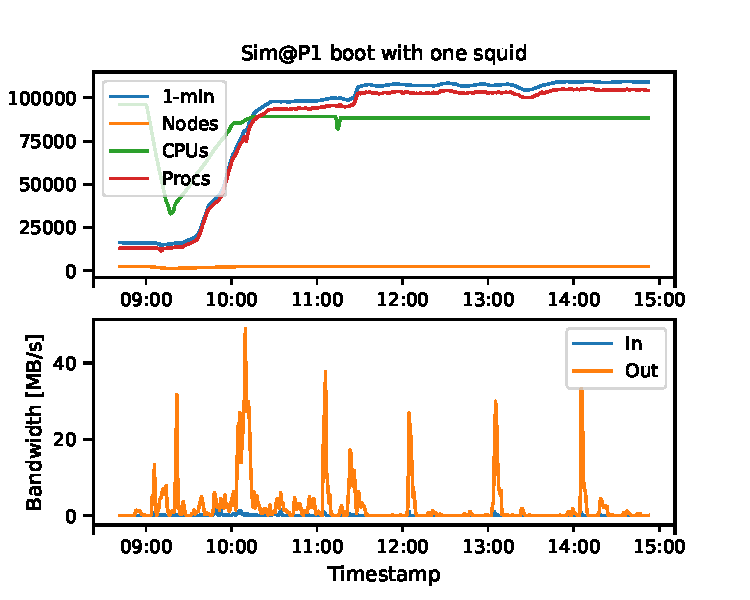
\includegraphics[width=0.6\textwidth,clip]{persistent_cache}
\caption{The top figure shows the number of instances, CPUs, and running
processes as well as the aggregate one minute load on the TDAQ HLT farm as it
transitions to offline mode. Below, using the same timestamps, the network load
on the two Frontier squids delivering the CVMFS content to all the nodes is
displayed. With the persistent cache the network traffic on the squids
is greatly reduced.}
\label{fig:persistent_cache}
\end{figure}
boots in the hour, with a slight time delay between the virtual machine being
created and being fully occupied with work.


\subsection{Squid hierarchy}
\label{sec:hierarchy}
As a complimentary approach to the persistent CVMFS caches the contextualisation
of the virtual machines was adjusted to run a squid in two instances in each
rack\footnote{The first and fifth TPU to ensure the squid proxy caches are in
separate chassis.}. The squids treat each other as siblings and the Frontier
squid
caches at P1 as parents. A web proxy-autodiscovery service is set up to
connect virtual machines to proxy caches on boot: those serving a squid
connect to the central Frontier squids at P1, others are connected to the two
squids in the same rack. Functionality was added to CernVM to delay the boot
process until at least one proxy cache is up.


\section{Operational experience}
\label{sec:ops}
The new configuration of Sim@P1 was operational within two days of the upgrade
to the TDAQ HLT. This quick transition is a testament to the simplification of
the Sim@P1 infrastructure under the new configuration. A feature of libvirt was
discovered when
returning the resources to HLT operation. The following section described the
workaround that was implemented. The squid hierarchy provided a marginal
improvement in the transition from online to offline operation while reducing
the
overall stability of the system: we started loosing racks when the two squids in
the rack cease functioning.

\subsection{Returning the resources}
\label{sec:return}
Should the virtual machine running on a TPU be busy with IO intensive
work\footnote{Usually an active application using swap space.} it may take some
time
for libvirt to destroy the virtual machine. Libvirt has a timeout of
15~\textrm{s} waiting
on the destruction of a virtual machine, taking longer produces an error in
returning that TPU to online mode. A helper script to manage the instance state
was written. It attempts to destroy the instance three
times, with a 15~\textrm{s} delay between attempts. With this modification all
resources were successfully returned to online mode on multiple occasion without
issues.

\subsection{Other workflows}
\label{sec:evgen}
Data taken by ATLAS is cached at point 1 and transferred to the CERN data centre
at the best rate the infrastructure can support. Tests performed at the end of
2018 have shown that we must assume the network between point 1 and CERN to be
busy transferring data from the cache to storage in the CERN data centre
during technical stops. Hence the restriction on the amount of data that can be
processed during offline operation remains.

Event generation is a frequent task that requires no input and produces very
little output. Previous experience with event generation found that depending on
the software used and the physics signal generated these tasks have a long tail
in the required memory. To explore the use of the Sim@P1 infrastructure for
event generation we created dedicated high memory and single core queues to test
various event generation tasks. At the end of 2019 first event generation tasks
were successfully executed on the Sim@P1 infrastructure. Since event generation
in ATLAS are workloads using a single core the four HTCondor schedulers were
fully occupied managing event generation reducing the overall usage of Sim@P1.

\subsection{Future improvements}
The infrastructure supporting Sim@P1 could be further improved to reduce the
work required to maintain the resource.

The legacy HLT hardware used permanently in
offline mode failed to reliably send heartbeats to PanDA when the system load
exceeds the available CPU cores. This
caused all work executing on these nodes to fail. To work around this we use the
``push\_noheartbeat'' workflow implemented by PanDA. The resources are returned
to online mode this mode causes jobs marked as running in PanDA to remain so for
48h. They must be removed manually. To automate this harvester could send
heartbeats for the jobs, similar to the the configuration used for HPC
facilities.

The success in running event generation in late 2019 shows that this could be
done in an automated setup. However workloads that greatly exceeding their
memory
allocation must be killed by HTCondor to ensure system stability. In addition,
additional HTCondor schedulers must be commissioned to accommodate the increased
number of jobs and limit the number of single core jobs allowed in the queue.

The hardware serving as Frontier squids operating at P1 needs to be replaced.
Supporting greater bandwidth for the CVMFS and Frontier content distribution
will further improve the rate at which the farm can be switched from HLT to
Sim@P1 mode. New hardware would mean the squid hierarchy described
in section~\ref{sec:hierarchy} could be removed improving the stability of
Sim@P1.

Longer term improvements would be using OpenStack's Heat or Kubernetes to build
and auto-scaling pool of HTCondor schedulers. Adding some volatile storage to
serve as a cache inside P1 may allow more data hungry workflows to be executed
without interfering with TDAQ operations\footnote{Such as Xcache of a volatile
Disk Pool Manager}.

\section{Conclusions}
The upgrade of the Sim@P1 hardware was swiftly and successfully accomplished at
the beginning of 2019. The new configuration is simpler and more robust since
it relies on low level Linux tools and libraries. The system has become much
more responsive by adding persistent CVMFS caches. More improvements promise to
make Sim@P1 more robust, versatile and easy to manage.


\begin{thebibliography}{}
  \bibitem{atlas}
   The ATLAS Collaboration
   %The  ATLAS  Experiment  at  the  CERN  Large  Hadron  Collider.
   JINST \textbf{3} S08003 (2008)

  \bibitem{tdaq2013}
  The ATLAS Collaboration, \textit{Technical Design Report for the Phase-I
  Upgrade of the ATLAS TDAQ System} (CERN, Geneva, 2013) 120-122

  %\cite{Ballestrero:2015ypa}
  \bibitem{Ballestrero:2015ypa}
    S.~Ballestrero {\it et al.}
    J.\ Phys.\ Conf.\ Ser.\  {\bf 664} 2  022008 (2015)
    %doi:10.1088/1742-6596/664/2/022008
    %%CITATION = doi:10.1088/1742-6596/664/2/022008;%%

  \bibitem{openstack}
    Openstack project, ”OpenStack” [software], version Icehouse, available from
    \url{https://www.openstack.org/software/icehouse/} [accessed 2018-09-24]

  \bibitem{Ballestrero:2017psv}
    S.~Ballestrero {\it et al.}
    %``Evolution and experience with the ATLAS Simulation at Point1 Project,''
    J.\ Phys.\ Conf.\ Ser.\  {\bf 898}  8 082012 (2017)
    %doi:10.1088/1742-6596/898/8/082012
    %%CITATION = doi:10.1088/1742-6596/898/8/082012;%%

    %\cite{Berghaus:2019wuj}
  \bibitem{Berghaus:2019wuj}
    F.~Berghaus {\it et al.} [ATLAS Collaboration],
    EPJ Web Conf.\  {\bf 214} (2019) 07021.
    %doi:10.1051/epjconf/201921407021
    %%CITATION = doi:10.1051/epjconf/201921407021;%%

  \bibitem{amiconfig}
    CernVM project, ``amiconfig'' [software], version cernvm-4, available from
    \url{https://github.com/cernvm/amiconfig} [accessed 2018-10-10]

  \bibitem{libvirt}
    libvirt project, ``libvirt virtualization API'' [software], version 0.10.2,
    available from \url{https://libvirt.org} [accessed 2018-10-10]

  \bibitem{condor}
    HTCondor project, ``HTCondor'' [software], version 8.6.11, available from
    \url{http://htcondor.org} [accessed 2018-09-24]

  \bibitem{harvester}
    PanDA project, ``Harvester'' [software], version 0.0.25, available from
    \url{https://github.com/PanDAWMS/panda-harvester} [accessed 2018-09-24]

  \bibitem{cernvm}
    CernVM team, ``CernVM'' [software], version 4.1, available from
    \url{http://cernvm.cern.ch} [accessed 2018-09-24]

\end{thebibliography}

\end{document}
